\chapter{Design und Verkleidung}

Da der Roboter künftig auf Hochschulveranstaltungen sowie weiteren Messen präsentiert werden soll, spielt neben der technischen Funktionalität auch sein äußeres Erscheinungsbild eine wesentliche Rolle. Aufbauend auf den Ergebnissen der vorangegangenen Arbeit wurde in dieser Arbeit ein maßgeblicher Fokus auf die Ausarbeitung eines stimmigen Designkonzeptes gelegt, das die Wiedererkennbarkeit der DHBW (PENDING LABEL) stärkt und gleichzeitig ein modernes sowie ansprechendes Erscheinungsbild gewährleistet.

\section{Entwicklung des Corporate Design}

Die Gestaltung eines Roboters umfasst nicht ausschließlich funktionale oder technische Aspekte, sondern beeinflusst maßgeblich die Wahrnehmung und Akzeptanz durch seine Nutzer. Insbesondere bei Robotern, die auf öffentlichen Veranstaltungen eingesetzt werden, dient das äußere Erscheinungsbild als wichtiges Kommunikationsmittel zwischen Mensch und Technik. Für den im Rahmen dieser Studienarbeit entwickelten Messe Roboter bestand das Ziel darin, ein Erscheinungsbild zu entwickeln, das sowohl die Corporate Design (PENDING LABEL) der DHBW (PENDING LABEL) widerspiegelt als auch auf Besucher unterschiedlicher Altersgruppen ansprechend wirkt.

Unter dem Begriff Corporate Design (PENDING LABEL) wird das einheitliche visuelle Erscheinungsbild einer Organisation verstanden. Es umfasst sämtliche gestalterischen Elemente wie Logo, Farbkonzept, Typografie und Bildsprache und dient dazu, einen konsistenten sowie wiedererkennbaren Außenauftritt zu gewährleisten. \cite{Helder.2026}

Ein wesentlicher Gestaltungsgrundsatz bestand darin, dem Roboter menschliche Merkmale zu verleihen, ohne dabei eine vollständig humanoide Erscheinung anzustreben. Zahlreiche Studien aus der Forschung zur Mensch-Roboter-Interaktion zeigen, dass Roboter mit einer leicht anthropomorphen, also an menschliche Merkmale angelehnten Gestaltung häufig als sympathischer, zugänglicher und vertrauenswürdiger wahrgenommen werden. Gleichzeitig kann eine zu starke Annäherung an das menschliche Erscheinungsbild zu einer gegenteiligen Wirkung führen. Dieses Phänomen wird als „Uncanny Valley” beschrieben. Dabei nimmt die Akzeptanz eines Roboters zunächst mit zunehmender Menschenähnlichkeit zu, sinkt jedoch deutlich ab, sobald der Roboter zwar fast menschlich wirkt, jedoch weiterhin erkennbare künstliche Eigenschaften besitzt. Dies kann bei Betrachtern Gefühle von Unbehagen oder Irritation hervorrufen. \cite{Uncanny.2026}

\vspace{1cm}
\begin{figure}[H]
	\centering
	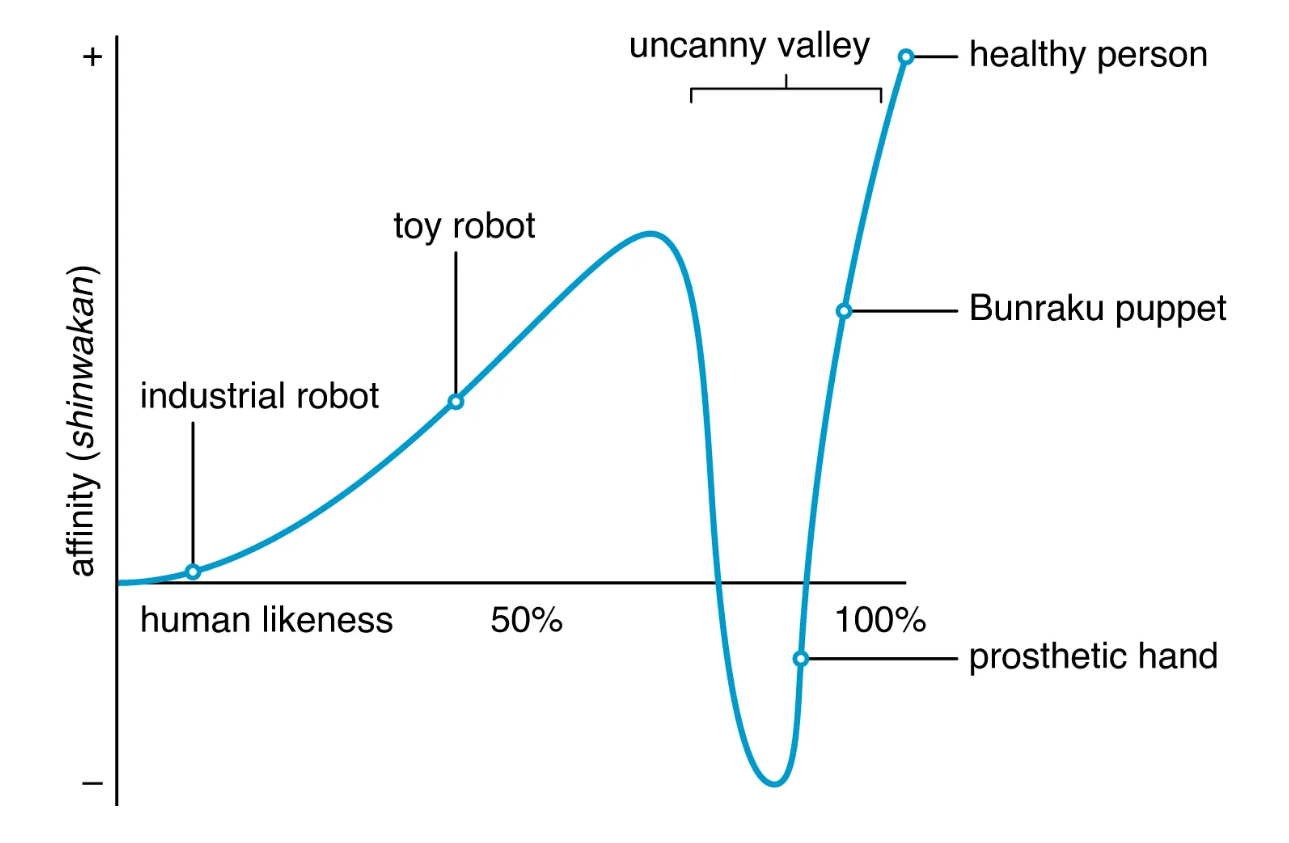
\includegraphics[width=0.8\linewidth]{images/uncannyvalley1.png}
	\vspace{10pt}
	\caption{Zeigt den „Uncanny Valley“ Effekt grafisch \cite{Mori.2012}}
	\label{fig:Uncanny}
\end{figure}

Das Diagramm in der Abbildung \ref{fig:Uncanny} zeigt, wie die Akzeptanz eines künstlichen Wesens mit zunehmender Menschenähnlichkeit verläuft. Auf der horizontalen Achse ist der Grad der „Human Likeness“ dargestellt. Er reicht von eindeutig maschinell generierten bis nahezu vollständig menschlichen Aussehen. Die vertikale Achse zeigt die „Affinity“, also wie positiv oder vertraut ein Objekt wahrgenommen wird. Zu Beginn steigt die positive Wahrnehmung, wobei einfache Industriemaschinen und Spielzeugroboter wirken vertraut. Sobald die Darstellung jedoch fast menschlich wirkt, fällt die Kurve deutlich ab. Dieser Bereich wird als „Uncanny Valley” bezeichnet. Figuren wie eine Prothesenhand lösen hier häufig Unbehagen aus. Erst bei nahezu perfekter Ähnlichkeit steigt die Akzeptanz wieder an.

Aus diesem Grund wurde bewusst auf eine realistische Nachbildung menschlicher Gesichtszüge oder Proportionen verzichtet. Stattdessen wurden lediglich ausgewählte anthropomorphe Elemente integriert, die den Roboter lebendig und freundlich erscheinen lassen, ohne Erwartungen an ein menschliches Verhalten zu erzeugen. Dazu zählen beispielsweise eine klar erkennbare Vorderseite, harmonische Proportionen sowie eine insgesamt freundliche Formensprache. Durch diese Gestaltung wird die Interaktion erleichtert, während gleichzeitig die technische Identität des Roboters erhalten bleibt.

Ein weiterer zentraler Aspekt ergab sich aus dem geplanten Einsatzgebiet. Das zu erwartende Publikum setzt sich aus Kindern, Jugendlichen, Eltern sowie Lehrkräften zusammen. Das Design muss daher unterschiedliche Zielgruppen gleichermaßen ansprechen. Während Kinder häufig auf auffällige Formen, freundliche Farben und einen spielerischen Charakter reagieren, erwarten fachkundige Besucher gleichzeitig einen professionellen und technisch hochwertigen Eindruck.

Vor diesem Hintergrund wurde ein Gestaltungskonzept entwickelt, das technische und spielerische Elemente miteinander kombiniert. Die Grundform des Roboters orientiert sich an einer modernen technischen Konstruktion und vermittelt Stabilität sowie Funktionalität. Gleichzeitig sorgen weiche Konturen, eine übersichtliche Gestaltung und eine reduzierte Formsprache für ein freundliches Erscheinungsbild. Dadurch entsteht ein ausgewogenes Verhältnis zwischen einem professionellen Demonstrationsobjekt und einem Roboter, der insbesondere bei jüngeren Messebesuchern Interesse und Neugier weckt.

Neben der allgemeinen Formgebung spielt die visuelle Identität der Dualen Hochschule Baden Württemberg eine entscheidende Rolle. Da der Roboter die Hochschule auf öffentlichen Veranstaltungen repräsentiert, muss seine Zugehörigkeit bereits auf den ersten Blick eindeutig erkennbar sein. Das Corporate Design (PENDING LABEL) erfüllt hierbei mehrere Funktionen. Einerseits schafft es einen hohen Wiedererkennungswert, andererseits stärkt es die Verbindung zwischen dem ausgestellten Robotersystem und der Hochschule als wissenschaftliche Einrichtung.

Aus diesem Grund wurden charakteristische Gestaltungselemente der Dualen Hochschule Baden Württemberg konsequent in das Design integriert. Hierzu zählen insbesondere das offizielle Hochschullogo sowie die typischen Farben der DHBW (PENDING LABEL). Die Positionierung dieser Elemente erfolgt an gut sichtbaren Bereichen des Roboters, sodass sie unabhängig vom Betrachtungswinkel möglichst deutlich wahrgenommen werden können. Gleichzeitig wurde darauf geachtet, das Erscheinungsbild nicht durch eine übermäßige Anzahl grafischer Elemente zu überladen. Stattdessen folgt das Gestaltungskonzept dem Grundsatz einer klaren und reduzierten visuellen Kommunikation.

Besondere Bedeutung besitzt die Wiedererkennbarkeit des Roboters innerhalb einer Messeumgebung. Solche Orte sind durch eine Vielzahl unterschiedlicher Messestände, Exponate und Besucher geprägt. Dadurch entsteht eine visuell stark belastete Umgebung, in der einzelne Objekte schnell an Aufmerksamkeit verlieren können. Um dennoch eine hohe Sichtbarkeit zu erreichen, muss sich der Roboter eindeutig von seiner Umgebung abheben und gleichzeitig eine unmittelbare Verbindung zur Dualen Hochschule Baden Württemberg herstellen.

Dieses Ziel wurde durch ein unverwechselbares Designkonzept verfolgt, bei dem Formgebung, Farbgestaltung und Markenkennzeichnung aufeinander abgestimmt wurden. Die charakteristischen Farben der Hochschule erzeugen bereits aus größerer Entfernung einen hohen Wiedererkennungswert. Ergänzend unterstützt das deutlich platzierte Hochschullogo die sofortige Identifikation des Roboters als Exponat der Dualen Hochschule Baden Württemberg. Durch die Kombination aus klarer Formensprache und markanter visueller Gestaltung bleibt der Roboter auch in einer stark frequentierten Messeumgebung gut wahrnehmbar.


\vspace{1cm}
\begin{figure}[H]
	\centering
	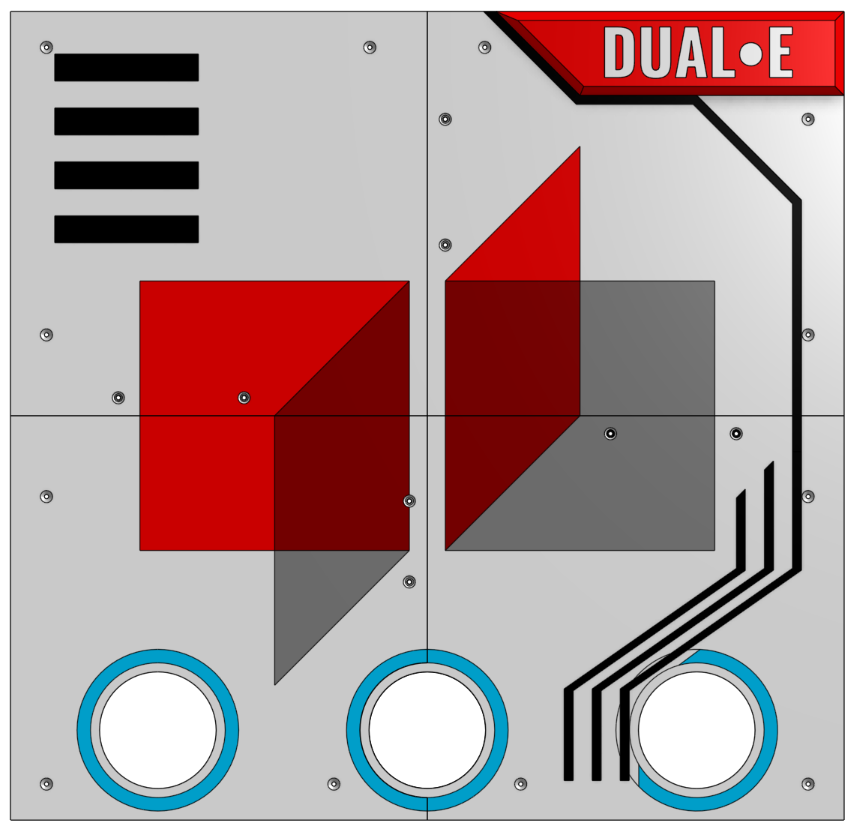
\includegraphics[width=0.7\linewidth]{images/DEFPV1.png}
	\vspace{15pt}
	\caption{Das CAD-Design der Frontplatte für den Roboter.}
	\label{fig:DEFPV1}
\end{figure}

Die Abbildung \ref{fig:DEFPV1} zeigt eine technische, futuristisch wirkende Frontplatte für die Verkleidung des Roboters. Die Platte besteht aus vier quadratischen Bereichen und ist durch sichtbare Schrauben, klare Linien und geometrische Formen strukturiert. Im Zentrum befindet sich markant das Logo der DHBW, das als visuelle Mitte dient und sofort Aufmerksamkeit erzeugt. Die Gestaltung nutzt kräftige Rot‑, Weiß- und Grautöne, die an das Erscheinungsbild der DHBW (PENDING LABEL SHORTS) erinnern und dem gesamten Panel eine eindeutige institutionelle Zuordnung geben. Rechts oben steht der Name „DUAL $\bullet$ E“, dessen Name an den fiktiven Roboter „WALL $\bullet$ E“ aus dem gleichnamigen Animationsfilm angelehnt ist, der dem Roboter eine eigene Identität verleiht und gleichzeitig spielerisch wirkt. Die horizontalen Linien im oberen linken Segment erinnern an technische Lüftungsschlitze und verleihen dem Design einen Charakter im Cyberpunk-Stil \cite{Linearity.2022}. Unten sind drei kreisförmige, hellblaue Markierungen platziert, die spätere Positionen von Ultraschallsensoren umschließen und damit eine funktionalere Ebene zeigen sollen, die über pure Markenoptik hinaus geht. 
Im gesammten Design werden verbindungen mit dem 
markenbezogenes Erscheinungsbild und klaren technischen Elementen durch diese hellblaue Fabmarkierung gekenzeichnet. Somit sollen diese technisch bzw. funktional relevanten Stellen klar gegenüber dem Design erkennbar sein. Mit dieser Makrierung der Technischen Funktionen soll der Roboter sowohl modern als auch professionell wirkt.


\vspace{1cm}
\begin{figure}[H]
	\centering
	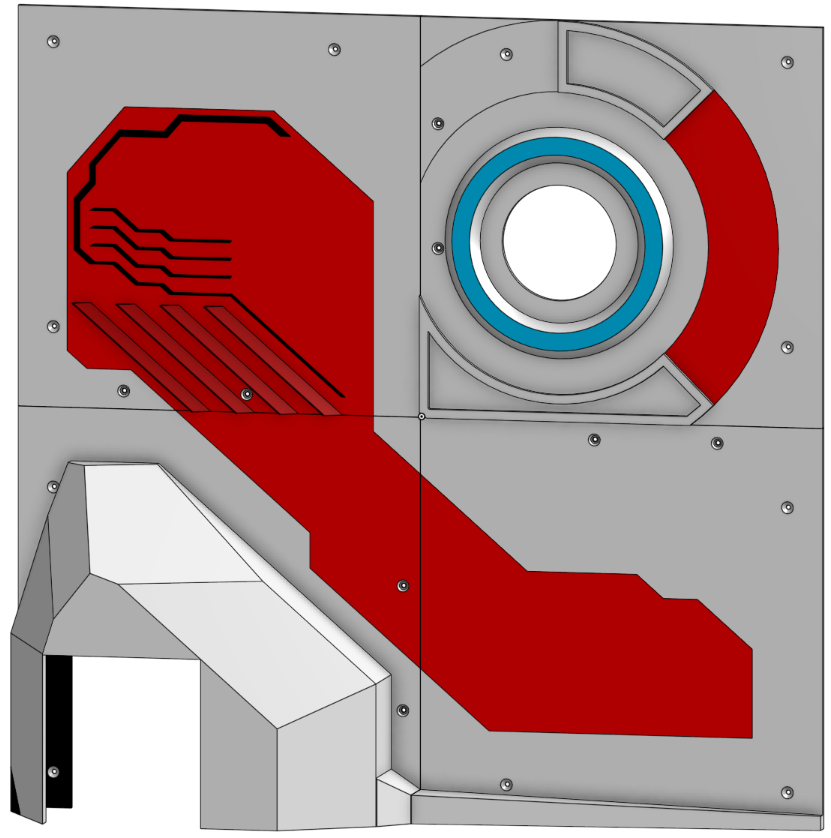
\includegraphics[width=0.7\linewidth]{images/DERPV1.png}
	\vspace{15pt}
	\caption{Das CAD-Design der rechten Platte für den Roboter.}
	\label{fig:DERPV1}
\end{figure}

Die Abbildung \ref{fig:DERPV1} zeigt die technisch‑futuristische Gestaltung von der rechte Design-Platte, die klar an das vorherige Design anknüpft, aber neue Akzente setzt. Die linke Platte sieht dementsprechend spiegelverkehrt aus. Die Seite ist in einem kräftigen Rot gehalten, das sofort ins Auge fällt und bewusst als schnelles Erkennungsmerkmal in belebten Umgebungen dient. Dieses Farbfeld unterstützt die Markenwirkung und sorgt dafür, dass der Roboter auch aus größerer Distanz eindeutig identifizierbar bleibt. Der kreisförmige Bereich mit helblauem Ring deutet den Einsatz der Arme an. Dadurch entsteht auch an dieser Stelle eine visuelle Verbindung zwischen der Platte und den funktionalen Komponenten des Roboters.

Der untere Bereich besitzt einen kantigen, massiv wirkenden Kotflügel für die Bedeckung der Räder, der an die Ästhetik eines 
%blockigen Schiffsrumpfs oder eines „Destroyer“-Designs erinnert 
militärischen Tarnkappenschiffs orientiert (siehe Abbildung \ref{fig:Destroyer}). Diese Gestaltung vermittelt Robustheit und technische Stärke, ohne übertrieben martialisch zu wirken. Insgesamt entsteht ein Panel, das sowohl funktionale Hinweise als auch markante Stilmerkmale vereint und den Roboter klar als modernes, technisch kompetentes System präsentiert.


\vspace{1cm}
\begin{figure}[H]
	\centering
	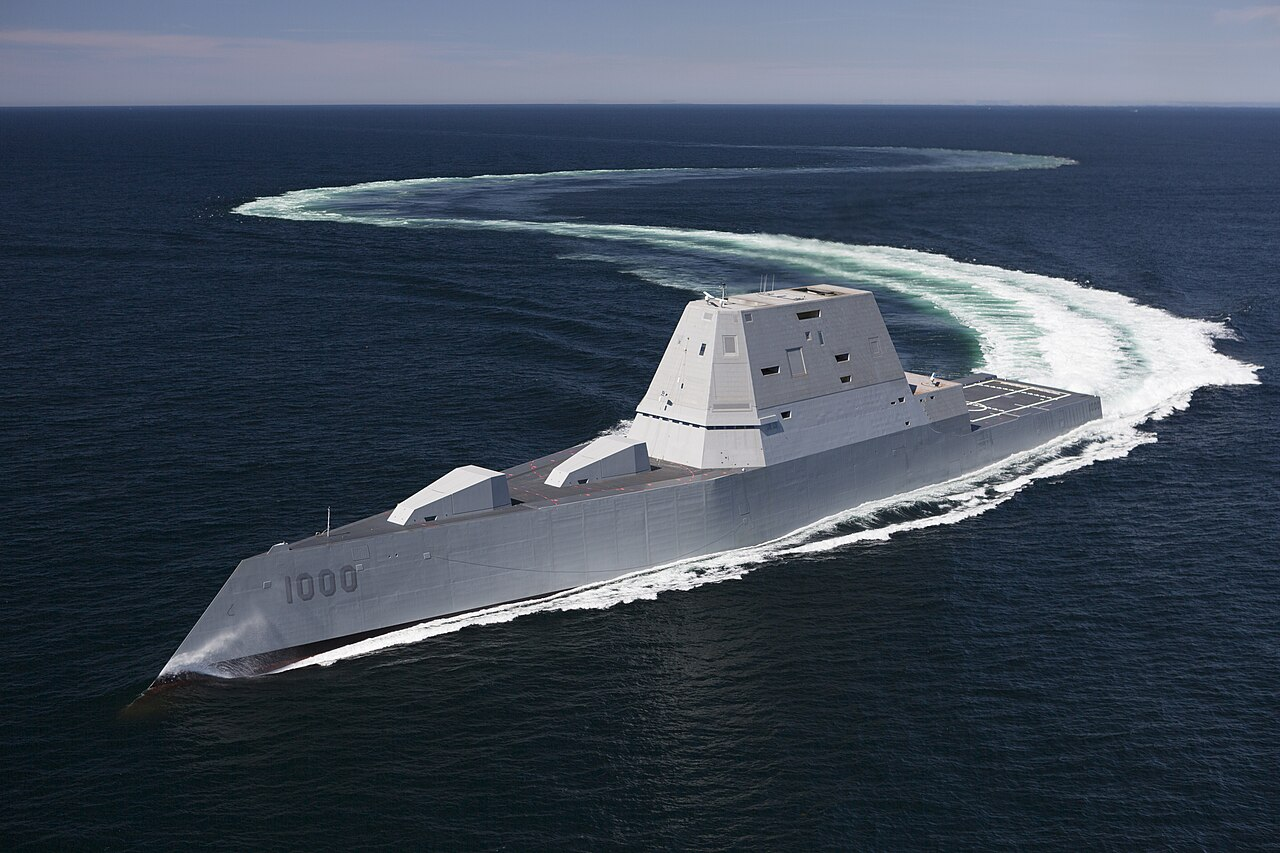
\includegraphics[width=0.6\linewidth]{images/USS_Zumwalt.jpg}
	\vspace{15pt}
	\caption{USS Zumwalt Schiff. \cite{Zumwalt.2016}}
	\label{fig:Destroyer}
\end{figure}

% PENDING WRITE ABOUT BACK PLATE, HOW ITS MORE TECHNICAL AND MOTORHAUBE (INKL BATTERIES???)

Für die hintere Platte steht die technische Funktion und Gestaltung im Vordergrund, da sie zentrale Komponenten schützt und den schnellen Zugriff auf die Batterie ermöglicht, ähnlich einer Motorhaube. 

%\vspace{1cm}
\begin{figure}[H]
	\centering
	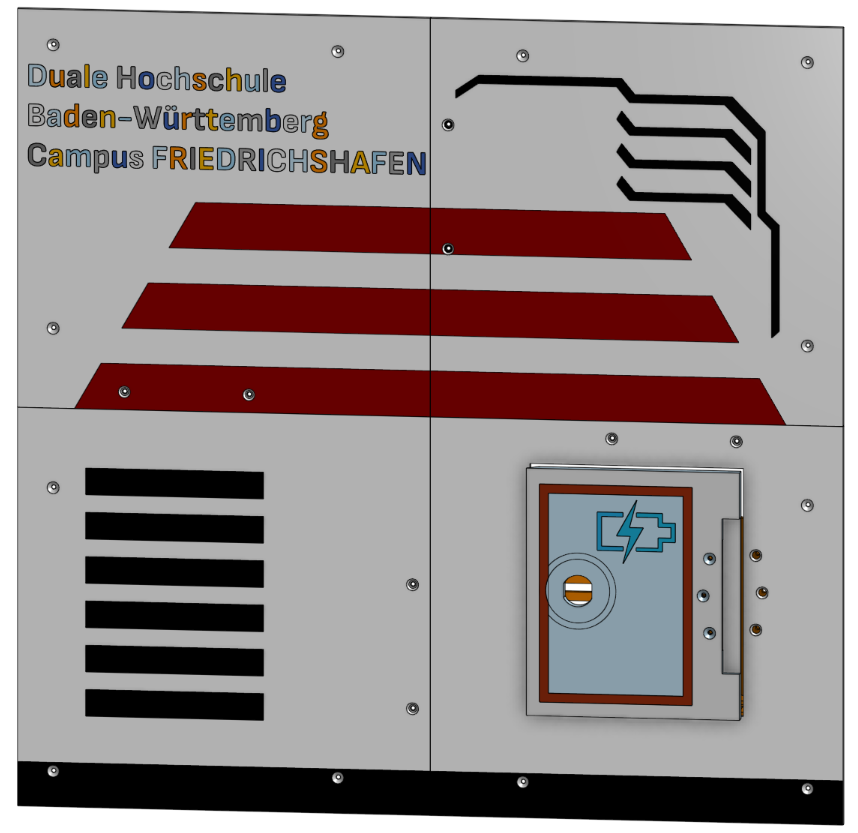
\includegraphics[width=0.7\linewidth]{images/DEBPV2.png}
	\vspace{15pt}
	\caption{Das CAD-Design der hinteren Platte „DEBPV2“ für den Roboter.}
	\label{fig:DEBPV2}
\end{figure}

Die gezeigte Platte in der Abbildung \ref{fig:DEBPV1} setzt genau diesen funktionalen Charakter sichtbar um. Die Platte trägt das Branding der DHBW klar und zentral, wodurch die Rückseite trotz technischer Ausrichtung eine eindeutige institutionelle Identität behält. Aus Gründen der Drucktechnik ist Branding als mehreren Teilen gekennzeichnet und ist somit mehrfarbig, wobei das Branding in gedruckten Form rot sein wird. Die roten Streifen auf der linken Seite dienen als visuelle Akzentführung und unterstützen die Wiedererkennbarkeit des Roboters, während die schwarzen Linien oben rechts an technische Leiterbahnen erinnern und den cyberpunkartigen Stil fortführen. Unten links sind Lüftungsschlitze integriert, die den technischen Charakter der Platte betonen. Rechts unten befindet sich eine kleine Wartungsklappe mit rundem Verschluss und einem Batteriesymbol, das den Zugangspunkt für den Batterieaustausch markiert. Die sichtbaren Schrauben entlang der Kanten verdeutlichen die modulare Bauweise und die robuste Befestigung der Verkleidung. 

Das Batteriesymbol ist in der selben helblauen Farbe gehalten, welche schon an vorherigen Bereichen sylistisch zur Markierung technisch relevanter Stellen benutzt wurde. Diese kommt damit auch dem Messepersonal zugute, das genau weiß an welcher Stelle die Batterie gewechselt werden kann.

\vspace{0.6cm}
\begin{figure}[H]
	\centering
	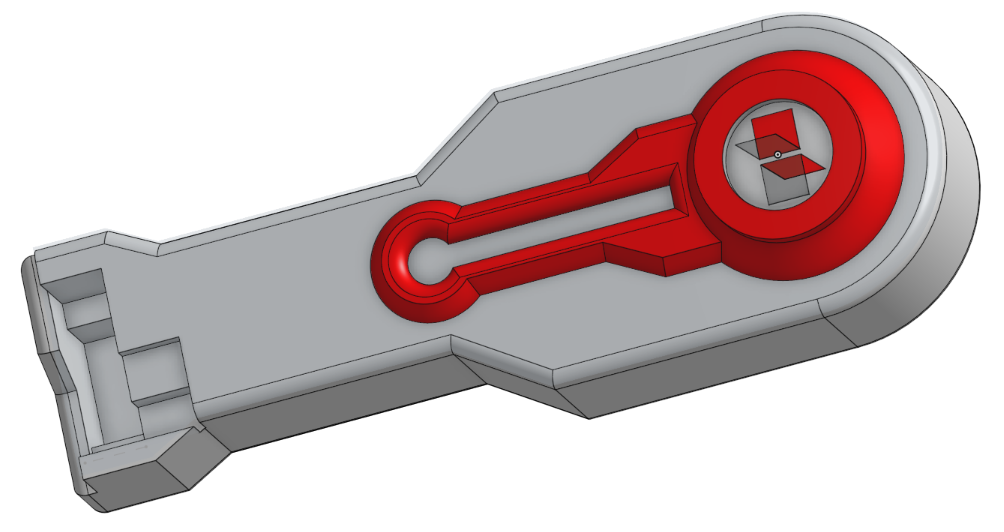
\includegraphics[width=0.7\linewidth]{images/DEArm1.png}
	\vspace{15pt}
	\caption{Das CAD-Design der Armverkleidung für dem Roboter.}
	\label{fig:DEArm1}
\end{figure}

Der Arm des Roboters in der Abbildung \ref{fig:DEArm1} besitzt die roten Akzentflächen und setzen somit die visuelle Linie der übrigen Verkleidung fort und sorgen dafür, dass der Arm auch als Teil des Gesamtfarbsystems erkennbar bleibt. Die Stelle an der der Arm gedreht wird, ist eine runde erhöhung, welche die posistion eines Schultergelenkes symbolisieren soll. Auf der Fläche dazwischen ist zudem das DHBW Logo eingearbeitet, was dem Bauteil eine eindeutige institutionelle Identität gibt und den Arm optisch mit den anderen Platten verbindet. Auf der linken Seite in der Abbildung \ref{fig:DEArm1} befindet sich der Bereich, in dem der Servomotor für die Klauen eingesetzt wird. Die Geometrie ist dort bewusst offen und funktional gehalten, damit der Motor sauber montiert werden kann.

%Die Arme bestehen dabei aus zwei schalenteilen, die einen Hohlen gesammtkörper ergeben. Dies ist eine technische Designentscheidung, die ermöglicht das sohwol material gespart werden kann, als auch um die Leitungen der Servomotoren für die Klauen hindurchzuführen. Die Klauen lassen sich mit ihren Servomotoren nur beim trennen der beiden schalen ausbauen, was verhindern soll, dass diese auf der Messe von unbefugten entwendet werden können.

Das entwickelte Corporate Design basiert auf der Kombination funktionaler, psychologischer und gestalterischer Anforderungen. Die bewusst begrenzte Anthropomorphisierung vermeidet die negativen Effekte des Uncanny Valley und fördert gleichzeitig eine positive Wahrnehmung des Roboters. Die ausgewogene Verbindung technischer und spielerischer Gestaltungselemente ermöglicht eine zielgruppengerechte Ansprache der Messebesucher. Gleichzeitig sorgt die konsequente Umsetzung des Corporate Designs der Dualen Hochschule Baden Württemberg für eine hohe Wiedererkennbarkeit sowie eine eindeutige Zuordnung des Roboters zur Hochschule. Dadurch übernimmt der Roboter nicht nur technische Aufgaben, sondern fungiert zugleich als repräsentatives Aushängeschild der Hochschule auf öffentlichen Veranstaltungen.

\section{Konstruktion und Fertigung}

Für die Herstellung der Verkleidungsplatten wurde ein additiver Fertigungsprozess mittels Fused Deposition Modeling (FDM, PENDING LABEL \& QUELLE) gewählt. Dafür kam ein 3D-Drucker des Typs Bambu Lab H2D zum Einsatz. Dieser verfügt über einen begrenzten Bauraum von 330 × 320 × 325 $mm^3$ (Breite × Tiefe × Höhe), wodurch die maximalen Abmessungen eines einzelnen Druckteils eingeschränkt sind. Da die für den Roboter entwickelten Verkleidungsplatten die verfügbaren Druckabmessungen überschreiten, voraussichtlich +450 × 3 × +450 $mm^3$ (Breite × Tiefe × Höhe), konnten die Bauteile nicht als einzelne Komponenten gefertigt werden. Aus diesem Grund wurde jede Seitenverkleidung bereits während der Konstruktionsphase in mehrere Teilsegmente unterteilt.

Die Analyse der Bauteilabmessungen ergab, dass eine Aufteilung jeder Verkleidungsplatte in vier Einzelteile eine wirtschaftliche und fertigungstechnisch geeignete Lösung darstellt. Durch diese Segmentierung konnten sämtliche Bauteile innerhalb des verfügbaren Bauraums positioniert und ohne zusätzliche Fertigungsschritte gedruckt werden. Die Abmessungen einer Teilplatte beträgt voraussichtlich 250 × 3 × 250 $mm^3$ (Breite × Tiefe × Höhe). Gleichzeitig ermöglicht die Aufteilung eine effizientere Ausnutzung des Druckvolumens sowie eine vereinfachte Nachbearbeitung der einzelnen Komponenten.

Die Zerlegung einer Verkleidungsplatte in mehrere Segmente erfordert jedoch geeignete Maßnahmen zur späteren Montage. Hierfür wurde ein Verbindungskonzept entwickelt, das die einzelnen Teilstücke nach dem Druck präzise zueinander positioniert und dauerhaft miteinander verbindet. Die Verbindungselemente wurden in Form von ineinandergreifenden Geometrien ausgeführt, die einem Puzzle-Prinzip ähneln. Durch diese Gestaltung können die einzelnen Segmente bereits während der Montage eindeutig ausgerichtet werden. Gleichzeitig wird das Risiko von Positionsfehlern reduziert, da die Verbindungselemente eine definierte Lage der Bauteile zueinander vorgeben.

Bei der Auslegung der Verbindungselemente mussten die fertigungstechnischen Eigenschaften des FDM-Druckverfahrens (PENDING LABEL) berücksichtigt werden. Aufgrund von Maßabweichungen, Materialschrumpfung und druckprozessbedingten Toleranzen können Bauteile nach dem Druck geringfügig von ihren theoretischen CAD-Abmessungen abweichen. Um dennoch eine problemlose Montage sicherzustellen, wurde zwischen den ineinandergreifenden Verbindungselementen eine Toleranz von 0,8 mm vorgesehen. Diese Toleranzzone gewährleistet, dass die einzelnen Segmente auch bei geringen Fertigungsabweichungen ohne übermäßigen Kraftaufwand zusammengefügt werden können.

Die Wahl der Toleranz stellt dabei einen Kompromiss zwischen Passgenauigkeit und Montierbarkeit dar. Eine zu geringe Toleranz könnte dazu führen, dass sich die Bauteile aufgrund unvermeidbarer Fertigungsabweichungen nicht vollständig zusammenfügen lassen. Eine zu große Toleranz würde hingegen die Positioniergenauigkeit reduzieren und die Stabilität der Verbindung negativ beeinflussen. Die gewählte Toleranz von 0,8 mm erwies sich als geeigneter Mittelweg zwischen diesen Anforderungen.

Neben der Toleranzgestaltung besitzt die Dimensionierung der Verbindungsflächen einen wesentlichen Einfluss auf die Stabilität der fertigen Verkleidung. Die Übergangsbereiche zwischen den einzelnen Segmenten wurden daher bewusst mit ausreichend großen Überlappungs- beziehungsweise Verbindungsflächen ausgeführt. Dadurch wird die Belastung nicht punktuell auf einzelne Schrauben konzentriert, sondern über größere Bereiche verteilt. Dies reduziert lokale Spannungen innerhalb des Kunststoffbauteils und erhöht die strukturelle Festigkeit der gesamten Konstruktion.

Die eigentliche Befestigung erfolgt über Schraubverbindungen. Nach dem Zusammenfügen der einzelnen Segmente werden diese mithilfe von Schrauben dauerhaft fixiert. Gegenüber einer reinen Klebeverbindung bietet dieses Verfahren mehrere Vorteile. Zum einen entsteht eine lösbare Verbindung, wodurch einzelne Segmente bei Beschädigungen oder konstruktiven Änderungen ausgetauscht werden können. Zum anderen ermöglicht die Schraubverbindung eine höhere mechanische Belastbarkeit und verbessert die Langzeitstabilität der gesamten Verkleidungsplatte.


Für die farbliche Gestaltung der Verkleidungsplatten wurden zwei unterschiedliche Fertigungsansätze betrachtet. Die erste Möglichkeit bestand darin, sämtliche Bauteile zunächst einfarbig zu drucken und die gewünschten Farbakzenten anschließend durch Lackieren mit Hilfe der Bedeckung mit Klettband zu realisieren. Die zweite Möglichkeit sah vor, die verschiedenen Farben bereits während des 3D-Druckprozesses durch den Einsatz unterschiedlich farbiger Filamente zu erzeugen.

Das nachträgliche Lackieren beziehungsweise Bekleben bietet den Vorteil, dass sämtliche Bauteile mit einem einzigen Filament gefertigt werden können. Dadurch reduziert sich der Aufwand während des Druckprozesses, da keine Filamentwechsel erforderlich sind und die Druckzeit insgesamt geringer ausfällt. Allerdings hängt die Qualität des Endergebnisses stark von der manuellen Ausführung ab. Insbesondere beim Abkleben und Lackieren können Ungenauigkeiten auftreten, wodurch Farbgrenzen unsauber werden oder die Positionierung einzelner Designelemente von der CAD-Konstruktion abweicht. Demgegenüber ermöglicht der mehrfarbige 3D-Druck eine deutlich höhere Präzision. Die verschiedenen Farben werden direkt während des Fertigungsprozesses an den zuvor definierten Positionen erzeugt, wodurch sich saubere Farbübergänge und eine hohe Wiederholgenauigkeit erzielen lassen. Dies ist insbesondere für die Umsetzung des Corporate Designs von Vorteil, da Logos, Schriftzüge und charakteristische Farbflächen exakt entsprechend der CAD-Konstruktion gefertigt werden können. Nachteile dieses Verfahrens bestehen in einer längeren Druckdauer aufgrund der erforderlichen Filamentwechsel sowie einem erhöhten Materialverbrauch, da bei jedem Farbwechsel Filament ausgespült werden muss.

Nach Abwägung beider Verfahren wurde entschieden, die Farbgestaltung direkt im 3D-Druckprozess umzusetzen. Obwohl dieses Verfahren mit einem höheren Zeit- und Materialaufwand verbunden ist, besitzt die präzise und reproduzierbare Umsetzung des Corporate Designs für den Messeeinsatz eine höhere Priorität. Dadurch kann sichergestellt werden, dass die Verkleidung den gestalterischen Anforderungen entspricht und ein hochwertiges sowie professionelles Erscheinungsbild des Roboters gewährleistet.

\vspace{1cm}
\begin{figure}[H]
	\centering
	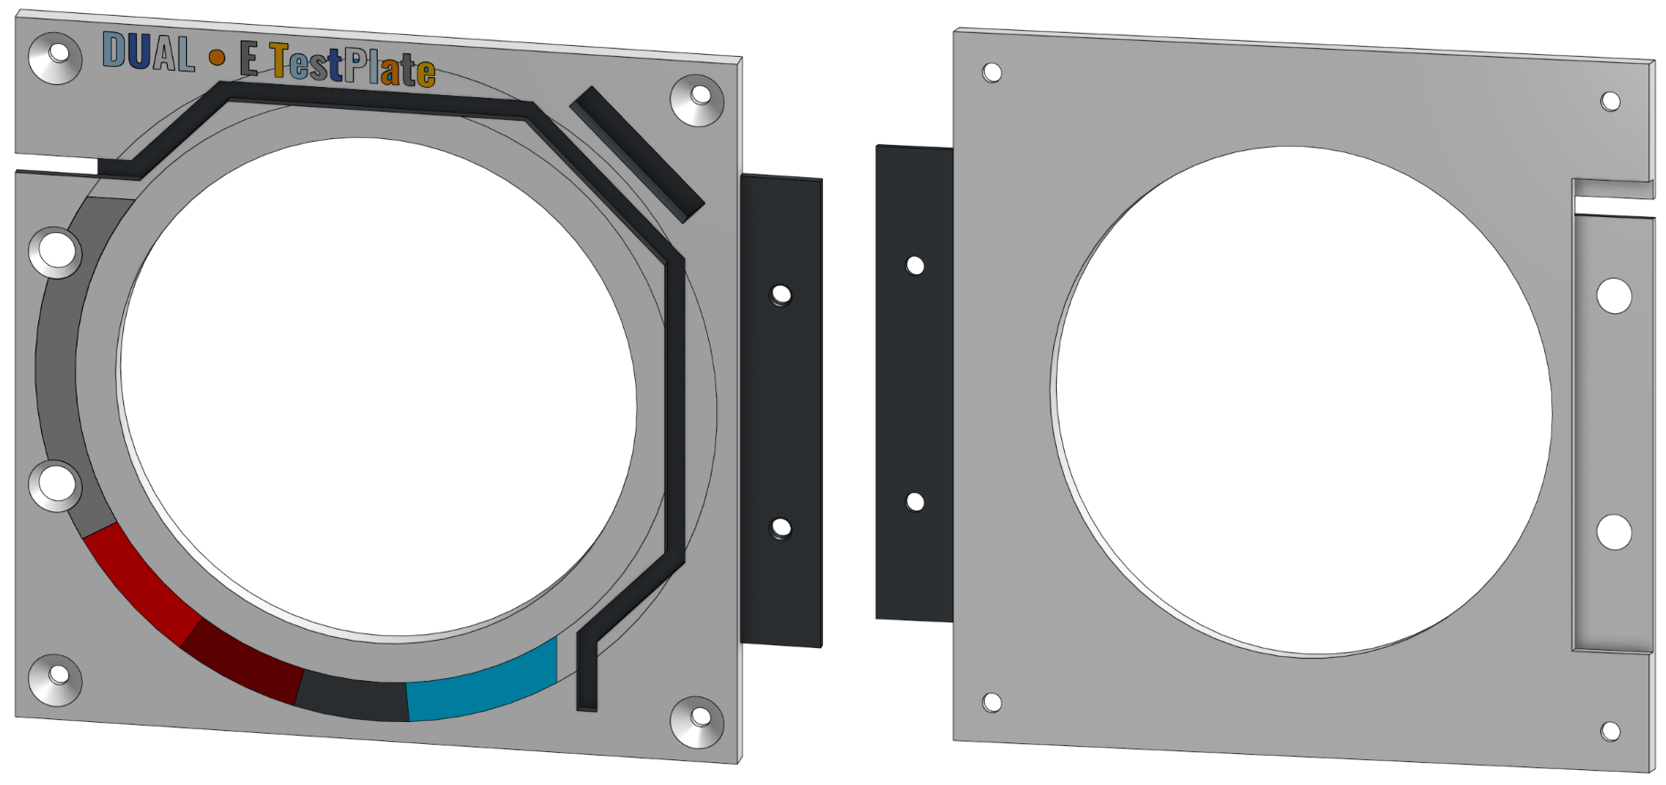
\includegraphics[width=0.9\linewidth]{images/TestPlate1.png}
	\vspace{20pt}
	\caption{Das CAD-Design der Testplatte für den Testdruck (links: vordere Seite, rechts: hintere Seite).}
	\label{fig:Testplatte}
\end{figure}


Die Testplatte, wie in der Abbildung \ref{fig:Testplatte} dargestellt, zeigt eine gestalterisch experimentelle Oberfläche, die speziell dafür ausgelegt ist, verschiedene Aspekte der Konstruktion und Fertigung zu prüfen. Links und rechts von der Testplatte erkennt man die mit bereits erwähnten Toleranz von 0,8 mm Verknüpfungsflächen, über die mehrere dieser Platten miteinander verbunden werden können. Die Schraubenlöcher sind in M3‑Normgröße ausgeführt und dienen in diesem Fall der Überprüfung der Passgenauigkeit im Druck. Die eingravierten Cyberpunk‑Linien besitzen eine leichte Tiefe, um zu testen, ob der Drucker feine Reliefstrukturen sauber reproduzieren kann. Zusätzlich sind mehrere Farbsegmente integriert, die als Drucktest dienen, mit der Vorgabe, dass während des Druckens maximal fünf unterschiedliche Farbabstufungen verwendet werden. Der große Kreis in der Mitte ist als Testaufnahme für Ultraschallsensoren vorgesehen und ermöglicht das Prüfen von Befestigung, Toleranzen und Stabilität. Ein kleines Text‑Label ist ebenfalls integriert, um die Lesbarkeit und Präzision von Schriftzügen im Druckprozess zu evaluieren.

Ebenso wurde die Position der Verbindungsflächen sorgfältig gewählt. Bereiche mit erhöhten mechanischen Belastungen oder möglichen Krafteinleitungen wurden bei der Segmentierung möglichst vermieden. Stattdessen erfolgte die Platzierung der Verbindungsstellen an konstruktiv günstigen Positionen, an denen die Belastungen geringer ausfallen und gleichzeitig ausreichend Bauraum für die Montage der Schraubverbindungen vorhanden ist. Dadurch konnte sowohl die mechanische Stabilität als auch die Wartungsfreundlichkeit verbessert werden.

\vspace{1cm}
\begin{figure}[H]
	\centering
	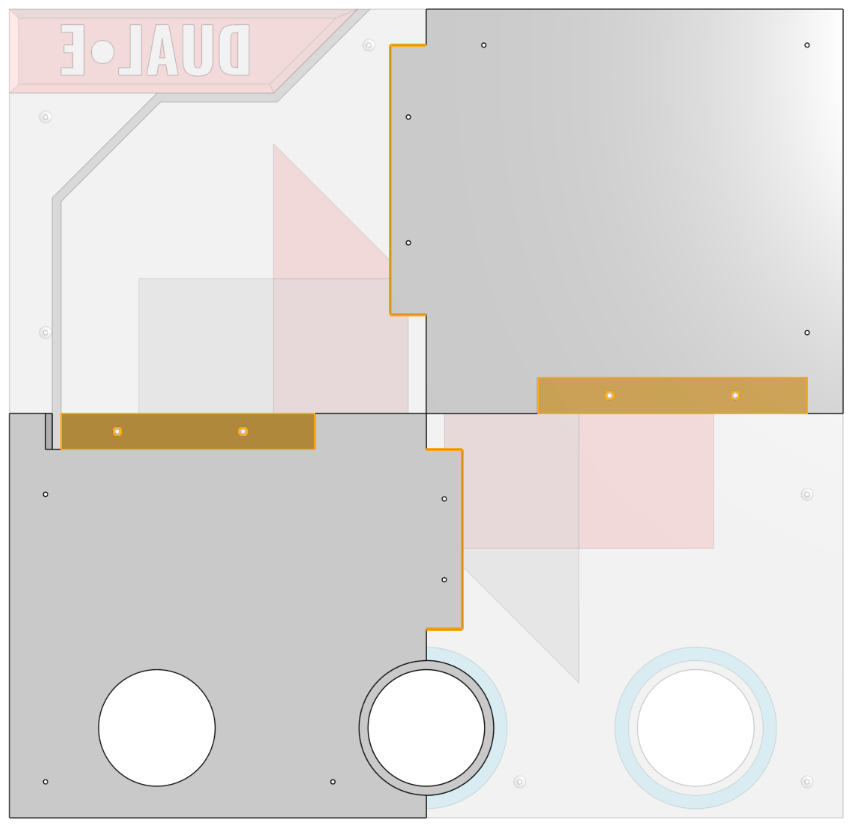
\includegraphics[width=0.7\linewidth]{images/DEFPV1_back.png}
	\vspace{20pt}
	\caption{Die Rückseite der Frontplatte „DEFPV1“ in transparenter Darstellung.}
	\label{fig:DEFPV1_back}
\end{figure}

Die Abbildung \ref{fig:DEFPV1_back} zeigt, wie die Verknüpfungsflächen in einer echten Verkleidungsplatte positioniert werden, hier exemplarisch auf der Rückseite der Frontplatte „DEFPV1“.  Die orange markierten Bereiche zeigen klar, wo die Verknüpfungsflächen sitzen. Die Flächen liegen breit verteilt über Außen- und Innenbereiche, sodass die Verbindung später sowohl außen als auch innen stabil bleibt. Gleichzeitig sind sie nicht exakt so breit wie die gesamte Teilplatte, damit beim Zusammenfügen mehrerer Module eine kleine Puzzle‑Lücke entsteht, die das Einrasten und Toleranzausgleichen ermöglicht. Die Schraublöcher sind nach M3‑Norm ausgeführt, sodass die Module zuverlässig fixiert werden können. Die kreisförmigen Aussparungen unten links deuten auf die spätere Integration von Ultraschallsensoren hin.

Nach Abschluss der Fertigung wurden die einzelnen Segmente zu vollständigen Verkleidungsplatten montiert und anschließend am Robotersystem befestigt. Durch die Kombination aus additiver Fertigung, segmentierter Bauweise und verschraubten Verbindungselementen entstand eine robuste und gleichzeitig flexibel anpassbare Konstruktion. Die gewählte Vorgehensweise ermöglichte die Herstellung großflächiger Verkleidungselemente trotz der begrenzten Abmessungen des verfügbaren 3D-Druckers.

Zusammenfassend stellte die Aufteilung der Verkleidungsplatten in vier Segmente eine zweckmäßige Lösung zur Umsetzung der großformatigen Bauteile dar. Das entwickelte Verbindungskonzept mit Puzzle-artigen Verbindungsgeometrien, verschraubten Verbindungen und definierten Toleranzbereichen gewährleistet eine präzise Montage sowie eine ausreichende mechanische Stabilität. Gleichzeitig ermöglicht die modulare Bauweise eine einfache Wartung und den Austausch einzelner Komponenten, wodurch die Flexibilität des Gesamtsystems erhöht wird.

\vspace{1cm}
\begin{figure}[H]
	\centering
	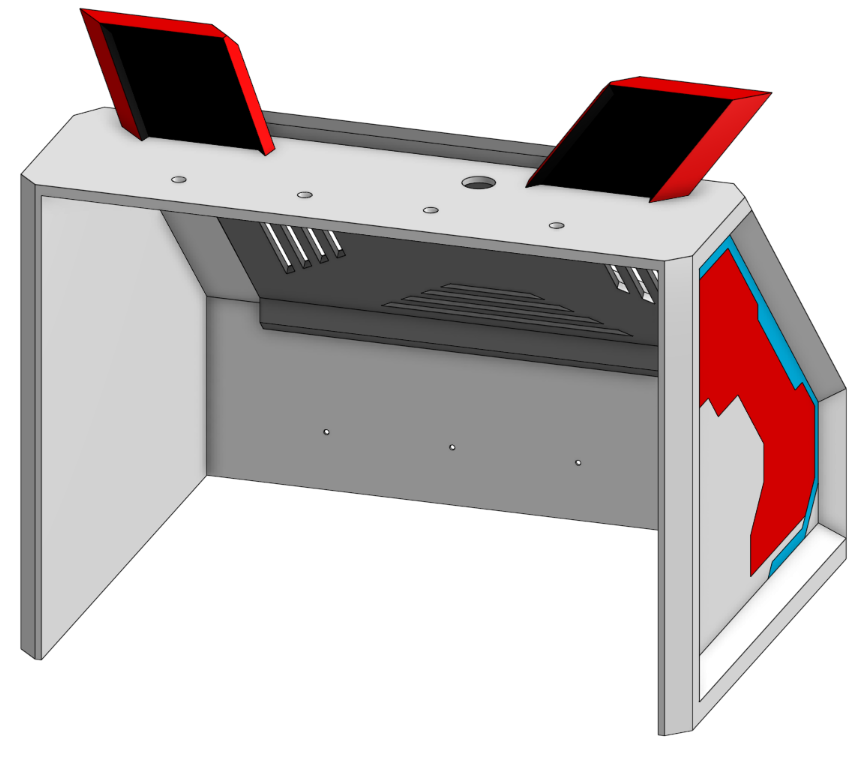
\includegraphics[width=0.7\linewidth]{images/DEHDV1.png}
	\vspace{15pt}
	\caption{Das CAD-Design der Verkleidung für dem Roboterkopf.}
	\label{fig:DEHDV1}
\end{figure}

Die Verkleidung für dem Roboterkopf, wie in der Abbildung \ref{fig:DEHDV1} dargestellt, wird als ein einziges Bauteil gefertigt, weil ihre Abmessungen problemlos innerhalb der Druckgröße des Bambu Lab H2C liegen. Dadurch entfällt jede Segmentierung, und die gesamte Form kann stabil, sauber und ohne sichtbare Übergänge gedruckt werden. Die M3‑Bohrungen sind direkt integriert, sodass alle späteren Befestigungen normgerecht und ohne Nacharbeit passen. Gestalterisch knüpft die Verkleidung an die übrigen Platten an. Die farblichen Akzentflächen sorgen für eine klare Verbindung zum Farbkonzept der anderen Platten und schaffen ein konsistentes Erscheinungsbild über den gesamten Roboter hinweg. Oben sitzen die „Ohren“, die bewusst als spielerisches Element gestaltet sind und dem Kopf eine leichte, freundliche Anmutung geben. Oben befindet sich ebenfalls ein größeres, ergonomisch platziertes Loch für einen Interaktionsknopf. Dieser liegt von der Draufsicht aus leicht rechts, weil Nutzer intuitiv häufiger mit der rechten Hand drücken. Die Position des Knopfes dient also nicht nur der Funktion, sondern folgt bewusst einer ergonomischen Platzierungslogik, damit die Interaktion mit dem Roboter möglichst natürlich wirkt.

\vspace{0.3cm}
\begin{figure}[H]
	\centering
	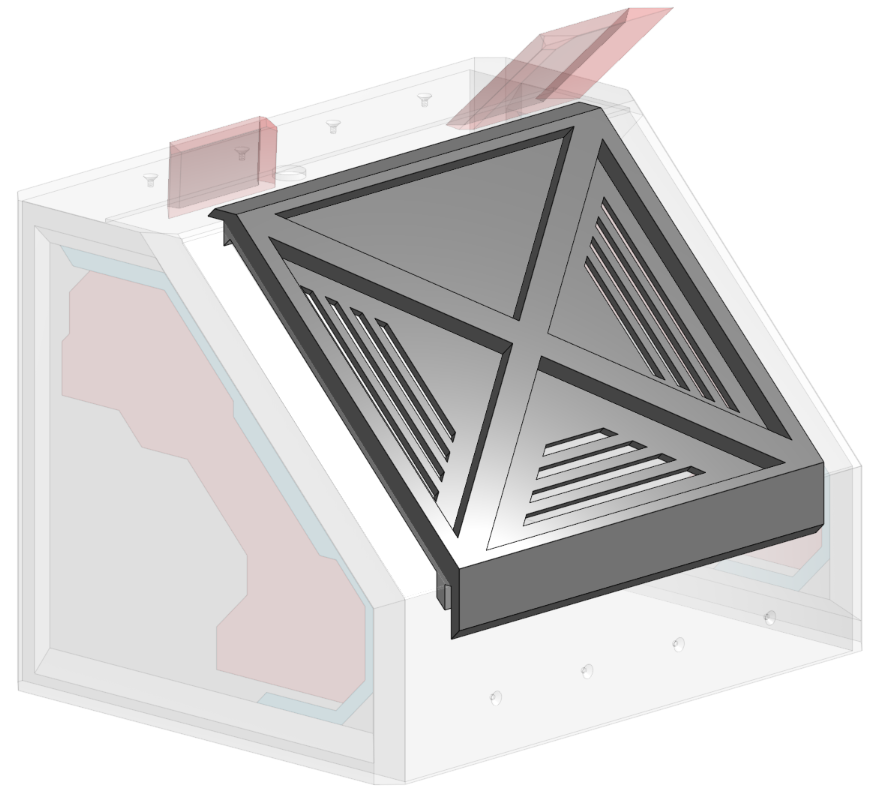
\includegraphics[width=0.7\linewidth]{images/DEHDV1_haube.png}
	\vspace{15pt}
	\caption{Das CAD-Design der Wartungsklappe für dem Roboterkopf, in die Verkleidung integriert.}
	\label{fig:DEHDV1_haube}
\end{figure}

Die Wartungsklappe,  wie in der Abbildung \ref{fig:DEHDV1_haube} dargestellt, ist als eigenständiges, funktionales Bauteil gestaltet und erfüllt mehrere technische Aufgaben gleichzeitig. Die Lüftungsschlitze sorgen dafür, dass alle Komponenten im Kopfbereich mit Luft versorgt werden und Wärme entweichen kann. %Sie sind so angeordnet, dass der Luftstrom möglichst gleichmäßig verteilt wird und keine Hotspots entstehen, was besonders bei kompakten Kopf‑Modulen wichtig ist.
Das große X‑Profil auf der Klappe dient als strukturelle Verstärkung. Durch diese Form wird die Fläche steifer und widerstandsfähiger. Die Klappe kann dadurch dünner konstruiert werden, ohne an Robustheit zu verlieren. Die untere und obere Schlitze sind außerdem so gestaltet, dass die Wartungsklappe ohne Schrauben oder Klebstoff auf der Verkleidung fixiert werden kann. Die Form greift seitlich und oben leicht genug ein, sodass man die Klappe einfach per Hand einsetzen oder herausnehmen kann. Gleichzeitig verhindern die Schlitze, dass die Klappe sich bei Bewegungen des Roboters seitlich verschiebt oder nach oben herausrutscht. Das ergibt eine werkzeuglose, aber sichere Befestigung, die bei Wartungsvorgängen praktisch ist.

\vspace{0.6cm}
\begin{figure}[H]
	\centering
	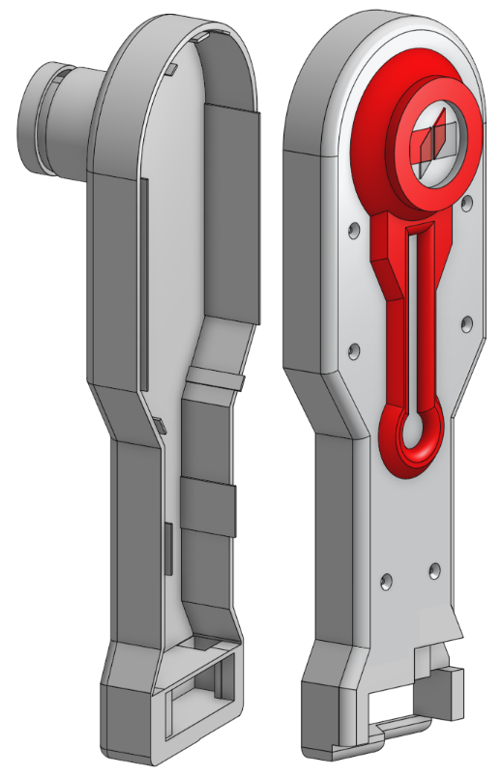
\includegraphics[width=0.5\linewidth]{images/DEArm2.png}
	\vspace{15pt}
	\caption{Die Armverkleidung in zwei Teile unterteilt.}
	\label{fig:DEArm2}
\end{figure}

Die Armverkleidung von der Abbildung \ref{fig:DEArm1} wird in zwei getrennte Teile unterteilt (siehe Abbildung \ref{fig:DEArm2}), die einen Hohlen gesammtkörper ergeben.
Dies ist eine technische Designentscheidung, die ermöglicht das sohwol material gespart werden kann, als auch um die Leitungen der Servomotoren für die Klauen hindurchzuführen. Montge und Wartung sind durch die Schalenbauweise besonders einfach. Die Klauen mit ihren Servomotoren (am Vorderen Ende des Armes) lassen sich  nur durch trennen der beiden Schalen ausbauen, was verhindern soll, dass diese auf der Messe von unbefugten entwendet werden können. 
Die auf der hinteren Arm-Schale zu erkennenden Nuten an der Innenseite (Abbildung \ref{fig:DEArm2}) ermöglich sauberes ineinandergreifen der beiden Hälften und verhinder verrutschen im festgeschraubten Zustand.

\vspace{1cm}
\begin{figure}[H]
	\centering
	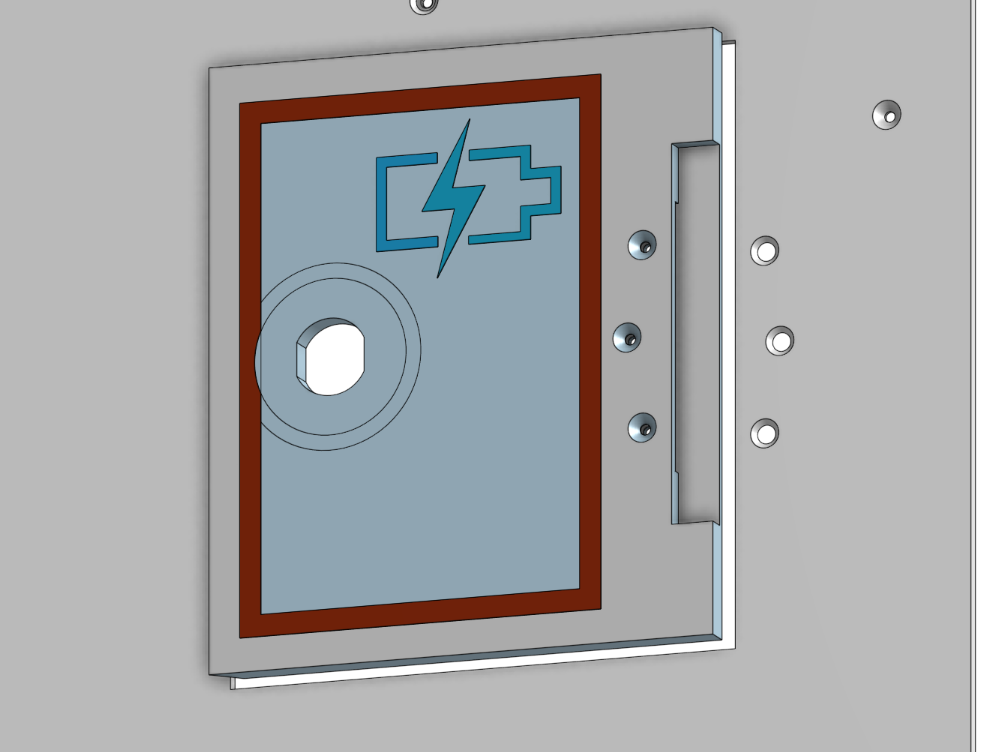
\includegraphics[width=0.7\linewidth]{images/DEBPV2_door.png}
	\vspace{15pt}
	\caption{Die Wartungsklappe von der hinteren Platte „DEBPV2“}
	\label{fig:DEBPV2_door}
\end{figure}

Die Abbildung \ref{fig:DEBPV2_door} stellt die Wartungsklappe von der hintere Verkleidungsplatte „DEBPV2“ genauer dar. Das runde Loch auf der linken Seite ist für den Einbau eines dreistelligen Zahlenschlosses vorgesehen. Die Geometrie ist so ausgelegt, dass das Schloss bündig sitzt und die Klappe zuverlässig verriegelt werden kann. Die Schraubenlöcher auf der rechten Seite dienen zur Befestigung der Klappe. Über diese Löcher wird die Klappe an der Verkleidungsplatte fixiert und gleichzeitig stabil gehalten. Zudem wird über diese Löcher ein Scharnier befestigt, sodass die Klappe geschwenkt werden kann. Die Form der Klappe und die Position der Schraubenlöcher sind darauf abgestimmt, dass das Scharnier sicher sitzt und die Klappe sich sauber öffnen und schließen lässt.

%\section{Elektronik-Design}
%
%\vspace{1cm}
%\begin{figure}[H]
%	\centering
%	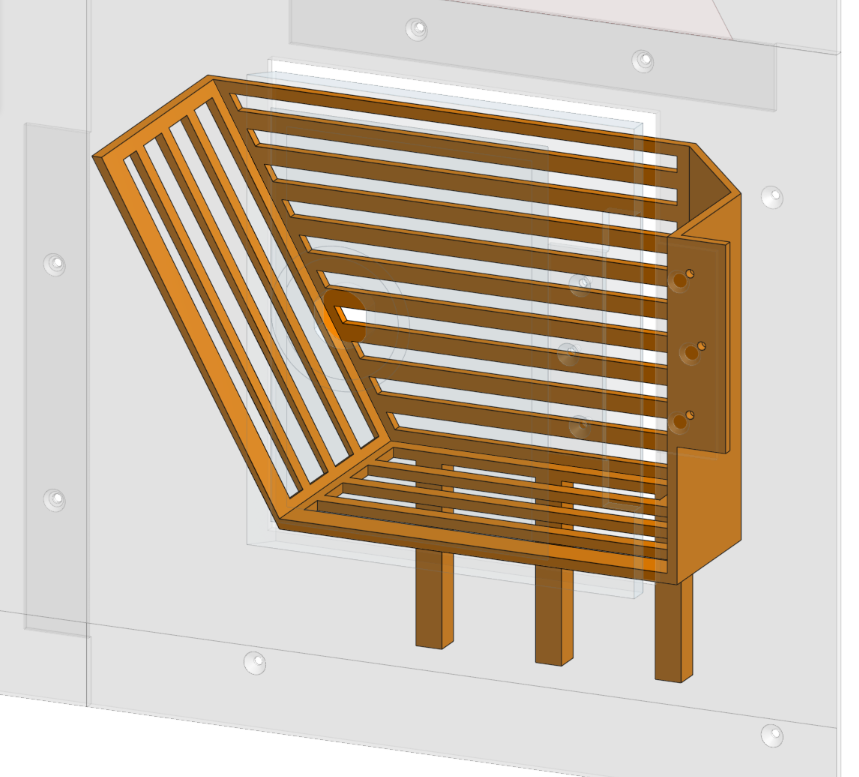
\includegraphics[width=0.8\linewidth]{images/BatteryTray.png}
%	\vspace{10pt}
%	\caption{Das CAD-Design der Batteriehalterung.}
%	\label{fig:BatteryTray}
%\end{figure}
%\textcolor{red}{Das wurde so nie eingebaut!}
%In der Abbildung \ref{fig:BatteryTray} wird die orangene Halterung für die Powerbanks im Inneren des Roboters dargestellt. Die Halterung sitzt direkt hinter der Wartungsklappe der hinteren Verkleidungsplatte (siehe Abbildung \ref{fig:DEBPV1}), sodass man die Powerbanks schnell erreichen und austauschen kann, ohne weitere Bauteile entfernen zu müssen. Die Befestigung ist bewusst effizient gelöst, in dem die gleichen M3‑Schrauben genutzt werden, die auch die Wartungsklappe und deren Scharniere halten. Dadurch bleibt die Konstruktion leicht, modular und ohne zusätzliche Verbindungspunkte. Die Struktur der Halterung ist mit Lüftungsschlitzen versehen. Diese dienen einerseits der Gewichtsreduktion, andererseits der Wärmeabfuhr, da Powerbanks unter Last spürbar warm werden können. Die Schlitze ermöglichen, dass warme Luft nach oben und hinten entweichen kann, während die Powerbanks sicher in ihrer Position bleiben. Die Anschlüsse an die Powerbank lassen sich ebenfalls duch die Schlitze ziehen.
